\documentclass[a4paper,10pt]{article}

\usepackage[english]{babel}
\usepackage{graphicx}
\usepackage[colorlinks, linkcolor=black, citecolor=black, urlcolor=black]{hyperref}
\usepackage{geometry}
\geometry{tmargin=3cm, bmargin=2.2cm, lmargin=2.2cm, rmargin=2cm}
\usepackage{todonotes} %Used for the figure placeholders

% Your name and student number must be filled in on the title page found in
% titlepage.tex.

\begin{document}
\begin{titlepage}
    \newpage
    \thispagestyle{empty}
    \frenchspacing
    \hspace{-0.2cm}
    
\includegraphics[height=3.4cm]{sedes}
    \hspace{0.2cm}
    \rule{0.5pt}{3.4cm}
    \hspace{0.2cm}
    \begin{minipage}[b]{8cm}
        \Large{Katholieke\newline Universiteit\newline Leuven}\smallskip\newline
        \large{}\smallskip\newline
        \textbf{Department of\newline Computer Science}\smallskip
    \end{minipage}
    \hspace{\stretch{1}}
    \vspace*{3.2cm}\vfill
    \begin{center}
        \begin{minipage}[t]{\textwidth}
            \begin{center}
                \LARGE{\rm{\textbf{\uppercase{Document Processing}}\\The
                complete architecture}}\\
                \Large{\rm{Software Architecture (H09B5a and H07Z9a) -- 
                Part 2b}}
            \end{center}
        \end{minipage}
    \end{center}
    \vfill
    \hfill\makebox[8.5cm][l]{%
        \vbox to 7cm{\vfill\noindent
            {\rm \textbf{Thomas Vochten (r0300128)}}\\
            {\rm \textbf{Frederik Goovaerts (r0256551)}}\\[2mm]
            {\rm Academic year 2014--2015}
        }
    }
\end{titlepage}


\tableofcontents
\newpage

\section{Domain analysis}\label{sec:domain}
\subsection{Domain models}
This section shows the domain model(s).

\begin{figure}[!htp]
    \centering
    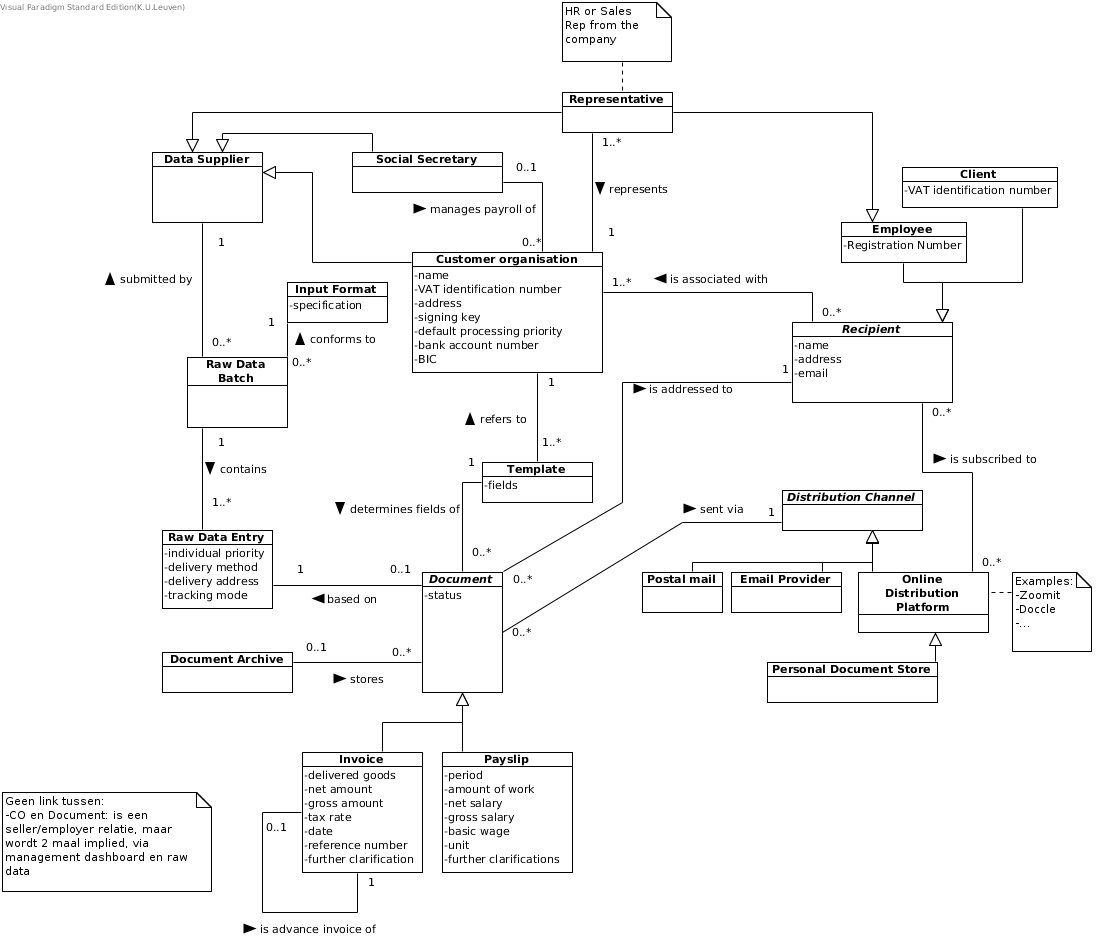
\includegraphics[width=0.8\textwidth]{domain_model.png}
    %\missingfigure[figwidth=0.8\textwidth]{Domain model}
    \caption{The domain model for the system.}\label{fig:domain_model}
\end{figure}

\subsection{Domain constraints}
In this section we provide additional domain constraints.

\begin{itemize}
    \item This is a first constraint.
    \item This is a second constraint.
\end{itemize}

\subsection{Glossary}
In this section, we provide a glossary of the most important terminology used
in this analysis.

\begin{itemize}
    \item \textbf{Term1}: definition
    \item \textbf{Term2}: definition
\end{itemize}

\section{Functional requirements}\label{sec:functional}
\subsection*{Use case model}

\begin{figure}[!htp]
    \centering
    %\includegraphics[width=0.8\textwidth]{}
    \missingfigure[figwidth=0.8\textwidth]{Use case model}
    \caption{Use case diagram for the system.}\label{fig:use_case_model}
\end{figure}

\subsection{\emph{UC7}: Filter documents in Personal Document Store}
\begin{itemize}
    \item \textbf{Primary actor:} Registered Recipient
    \item \textbf{Interested parties:} 
        \begin{itemize}
            \item \textit{eDocs:} Wants to know popular searches for optimising document caching
        \end{itemize}

    \item \textbf{Preconditions:}
        \begin{itemize}
            \item User has consulted his personal document store (UC4).
        \end{itemize}

    \item \textbf{Postconditions:}
        \begin{itemize}
            \item The Registered Recipient has received a new view of documents in his Personal document store, matching the query he gave to the system.
        \end{itemize}
        
    \item \textbf{Main scenario:} 
    \begin{enumerate}
       \item The user indicates he wants to pose a filter query to the Personal Document Store
       \item The user receives a form with filter choices, which he completes, and indicates he wants to filter with given parameters.
       \item The System retrieves all documents of the Registered User matching his query.
       \item The System provides an overview of all retrieved documents matching the User's query.
    \end{enumerate}

    \item \textbf{Alternative scenarios:} 
    \begin{enumerate}
        \item [4a.] The System did not find any documents matching the User's query
        \item [5a.] The Registered User receives a notification that no documents have matched his filter parameters.
    \end{enumerate}
    
    \item \textbf{Remarks:}
        \begin{itemize}
            \item Abstraction is made of the contents of the filter form. The given choices can be free form or very simple ones.
        \end{itemize}
\end{itemize}

\subsection{\emph{UC8}: Consult Document Delivery status}
\begin{itemize}
    \item \textbf{Primary actor:} Customer Organisation Representative
    \item \textbf{Interested parties:} 
        \begin{itemize}
            \item \textit{eDocs:} wants to let the organisation know their documents are actually being delivered
        \end{itemize}

    \item \textbf{Preconditions:}
        \begin{itemize}
            \item The Representative is logged in (UC1).
        \end{itemize}

    \item \textbf{Postconditions:}
        \begin{itemize}
            \item Representative has received Delivery information regarding the documents he is interested in.
        \end{itemize}
        
    \item \textbf{Main scenario:} 
    \begin{enumerate}
       \item The Representative signals he wants an overview of the company documents to which he has access (see remarks).
       \item The System retrieves all documents managed by the Representative.
       \item The System presents the Representative with an overview of the matching documents, including a small individual note per document whether it has been delivered or not.
       \item The use case ends here.
    \end{enumerate}

    \item \textbf{Alternative scenarios:} 
    \begin{enumerate}
        \item [4a.] The Representative indicates he wants to see details (see remarks) of a document present in the overview.
        \item [5a.] The System presents the Representative with the detailed information for indicated document.
        \item [4b.] The Representative indicates he only wants to see undelivered documents.
        \item [5b.] The System retrieves all undelivered documents managed by the Representative.
        \item [6b.] The System presents the Representative with an overview of the retrieved documents.
    \end{enumerate}
    
    \item \textbf{Remarks:}
        \begin{itemize}
            \item A representative only has access to documents generated by his role in the company. E.g. Sales representatives cannot consult payslips, which are managed by Human Resources Representatives.
            \item A document in an online distribution platform is only flagged as delivered after the document has also been opened by the Recipient.
            \item Details of a document in this Use Case denote for example the chosen distribution channel, the contents of the document, the date of generation \ldots
        \end{itemize}
\end{itemize}

\subsection{\emph{UC9}: Name of use case 9}
\begin{itemize}
    \item \textbf{Primary actor:} primary actor
    \item \textbf{Interested parties:} 
        \begin{itemize}
            \item \textit{Name of interested party:} reason why party is interested
        \end{itemize}

    \item \textbf{Preconditions:}
        \begin{itemize}
            \item First precondition.
            \item Second precondition.
        \end{itemize}

    \item \textbf{Postconditions:}
        \begin{itemize}
            \item First postcondition.
            \item Second postcondition.
        \end{itemize}
        
    \item \textbf{Main scenario:} 
    \begin{enumerate}
       \item Step 1
       \item Step 2
       \item Step 3
       \item \ldots
    \end{enumerate}

    \item \textbf{Alternative scenarios:} 
    \begin{enumerate}
        \item [3b.] Alternative at step 3
    \end{enumerate}
    
    \item \textbf{Remarks:}
        \begin{itemize}
            \item First remark
        \end{itemize}
\end{itemize}

\subsection{\emph{UC10}: Name of use case 10}
\begin{itemize}
    \item \textbf{Primary actor:} primary actor
    \item \textbf{Interested parties:} 
        \begin{itemize}
            \item \textit{Name of interested party:} reason why party is interested
        \end{itemize}

    \item \textbf{Preconditions:}
        \begin{itemize}
            \item First precondition.
            \item Second precondition.
        \end{itemize}

    \item \textbf{Postconditions:}
        \begin{itemize}
            \item First postcondition.
            \item Second postcondition.
        \end{itemize}
        
    \item \textbf{Main scenario:} 
    \begin{enumerate}
       \item Step 1
       \item Step 2
       \item Step 3
       \item \ldots
    \end{enumerate}

    \item \textbf{Alternative scenarios:} 
    \begin{enumerate}
        \item [3b.] Alternative at step 3
    \end{enumerate}
    
    \item \textbf{Remarks:}
        \begin{itemize}
            \item First remark
        \end{itemize}
\end{itemize}

\subsection{\emph{UC11}: Name of use case 11}
\begin{itemize}
    \item \textbf{Primary actor:} primary actor
    \item \textbf{Interested parties:} 
        \begin{itemize}
            \item \textit{Name of interested party:} reason why party is interested
        \end{itemize}

    \item \textbf{Preconditions:}
        \begin{itemize}
            \item First precondition.
            \item Second precondition.
        \end{itemize}

    \item \textbf{Postconditions:}
        \begin{itemize}
            \item First postcondition.
            \item Second postcondition.
        \end{itemize}
        
    \item \textbf{Main scenario:} 
    \begin{enumerate}
       \item Step 1
       \item Step 2
       \item Step 3
       \item \ldots
    \end{enumerate}

    \item \textbf{Alternative scenarios:} 
    \begin{enumerate}
        \item [3b.] Alternative at step 3
    \end{enumerate}
    
    \item \textbf{Remarks:}
        \begin{itemize}
            \item First remark
        \end{itemize}
\end{itemize}

\subsection{\emph{UC12}: Name of use case 12}
\begin{itemize}
    \item \textbf{Primary actor:} primary actor
    \item \textbf{Interested parties:} 
        \begin{itemize}
            \item \textit{Name of interested party:} reason why party is interested
        \end{itemize}

    \item \textbf{Preconditions:}
        \begin{itemize}
            \item First precondition.
            \item Second precondition.
        \end{itemize}

    \item \textbf{Postconditions:}
        \begin{itemize}
            \item First postcondition.
            \item Second postcondition.
        \end{itemize}
        
    \item \textbf{Main scenario:} 
    \begin{enumerate}
       \item Step 1
       \item Step 2
       \item Step 3
       \item \ldots
    \end{enumerate}

    \item \textbf{Alternative scenarios:} 
    \begin{enumerate}
        \item [3b.] Alternative at step 3
    \end{enumerate}
    
    \item \textbf{Remarks:}
        \begin{itemize}
            \item First remark
        \end{itemize}
\end{itemize}

\subsection{\emph{UC13}: Name of use case 13}
\begin{itemize}
    \item \textbf{Primary actor:} primary actor
    \item \textbf{Interested parties:} 
        \begin{itemize}
            \item \textit{Name of interested party:} reason why party is interested
        \end{itemize}

    \item \textbf{Preconditions:}
        \begin{itemize}
            \item First precondition.
            \item Second precondition.
        \end{itemize}

    \item \textbf{Postconditions:}
        \begin{itemize}
            \item First postcondition.
            \item Second postcondition.
        \end{itemize}
        
    \item \textbf{Main scenario:} 
    \begin{enumerate}
       \item Step 1
       \item Step 2
       \item Step 3
       \item \ldots
    \end{enumerate}

    \item \textbf{Alternative scenarios:} 
    \begin{enumerate}
        \item [3b.] Alternative at step 3
    \end{enumerate}
    
    \item \textbf{Remarks:}
        \begin{itemize}
            \item First remark
        \end{itemize}
\end{itemize}

\subsection{\emph{UC14}: Name of use case 14}
\begin{itemize}
    \item \textbf{Primary actor:} primary actor
    \item \textbf{Interested parties:} 
        \begin{itemize}
            \item \textit{Name of interested party:} reason why party is interested
        \end{itemize}

    \item \textbf{Preconditions:}
        \begin{itemize}
            \item First precondition.
            \item Second precondition.
        \end{itemize}

    \item \textbf{Postconditions:}
        \begin{itemize}
            \item First postcondition.
            \item Second postcondition.
        \end{itemize}
        
    \item \textbf{Main scenario:} 
    \begin{enumerate}
       \item Step 1
       \item Step 2
       \item Step 3
       \item \ldots
    \end{enumerate}

    \item \textbf{Alternative scenarios:} 
    \begin{enumerate}
        \item [3b.] Alternative at step 3
    \end{enumerate}
    
    \item \textbf{Remarks:}
        \begin{itemize}
            \item First remark
        \end{itemize}
\end{itemize}

\subsection{\emph{UC15}: Name of use case 15}
\begin{itemize}
    \item \textbf{Primary actor:} primary actor
    \item \textbf{Interested parties:} 
        \begin{itemize}
            \item \textit{Name of interested party:} reason why party is interested
        \end{itemize}

    \item \textbf{Preconditions:}
        \begin{itemize}
            \item First precondition.
            \item Second precondition.
        \end{itemize}

    \item \textbf{Postconditions:}
        \begin{itemize}
            \item First postcondition.
            \item Second postcondition.
        \end{itemize}
        
    \item \textbf{Main scenario:} 
    \begin{enumerate}
       \item Step 1
       \item Step 2
       \item Step 3
       \item \ldots
    \end{enumerate}

    \item \textbf{Alternative scenarios:} 
    \begin{enumerate}
        \item [3b.] Alternative at step 3
    \end{enumerate}
    
    \item \textbf{Remarks:}
        \begin{itemize}
            \item First remark
        \end{itemize}
\end{itemize}

\subsection{\emph{UC16}: Name of use case 16}
\begin{itemize}
    \item \textbf{Primary actor:} primary actor
    \item \textbf{Interested parties:} 
        \begin{itemize}
            \item \textit{Name of interested party:} reason why party is interested
        \end{itemize}

    \item \textbf{Preconditions:}
        \begin{itemize}
            \item First precondition.
            \item Second precondition.
        \end{itemize}

    \item \textbf{Postconditions:}
        \begin{itemize}
            \item First postcondition.
            \item Second postcondition.
        \end{itemize}
        
    \item \textbf{Main scenario:} 
    \begin{enumerate}
       \item Step 1
       \item Step 2
       \item Step 3
       \item \ldots
    \end{enumerate}

    \item \textbf{Alternative scenarios:} 
    \begin{enumerate}
        \item [3b.] Alternative at step 3
    \end{enumerate}
    
    \item \textbf{Remarks:}
        \begin{itemize}
            \item First remark
        \end{itemize}
\end{itemize}

\section{Non-functional requirements}\label{sec:non-functional}
In this section, we model the non-functional requirements for the system in the
form of \emph{quality attribute scenarios}. We provide for each type
(availability, performance and modifiability) one requirement.

\subsection{Availability}
\subsubsection{\emph{Av1}: Name of the quality attribute scenario}
Shortly describe the context of the scenario.

\begin{itemize}
    \item \textbf{Source:} source
    \item \textbf{Stimulus:}
        \begin{itemize}
            \item Description of a first stimulus.
            \item Description of a second stimulus.
        \end{itemize}

    \item \textbf{Artifact:} the stimulated artifact
    \item \textbf{Environment:} the condition under which the stimulus occurs
    \item \textbf{Response:}
        \begin{itemize}
            \item Describe how the system should respond to the stimulus.
        \end{itemize}

    \item \textbf{Response measure:}
        \begin{itemize}
            \item Describe how the satisfaction of a response is measured.
        \end{itemize}
\end{itemize}

\subsection{Performance}
\subsubsection{\emph{P1}: Name of the quality attribute scenario}
Shortly describe the context of the scenario.

\begin{itemize}
    \item \textbf{Source:} source
    \item \textbf{Stimulus:}
        \begin{itemize}
            \item Description of a first stimulus.
            \item Description of a second stimulus.
        \end{itemize}

    \item \textbf{Artifact:} the stimulated artifact
    \item \textbf{Environment:} the condition under which the stimulus occurs
    \item \textbf{Response:}
        \begin{itemize}
            \item Describe how the system should respond to the stimulus.
        \end{itemize}

    \item \textbf{Response measure:}
        \begin{itemize}
            \item Describe how the satisfaction of a response is measured.
        \end{itemize}
\end{itemize}

\subsection{Modifiability}
\subsubsection{\emph{M1}: Name of the quality attribute scenario}
Shortly describe the context of the scenario.

\begin{itemize}
    \item \textbf{Source:} source
    \item \textbf{Stimulus:}
        \begin{itemize}
            \item Description of a first stimulus.
            \item Description of a second stimulus.
        \end{itemize}

    \item \textbf{Artifact:} the stimulated artifact
    \item \textbf{Environment:} the condition under which the stimulus occurs
    \item \textbf{Response:}
        \begin{itemize}
            \item Describe how the system should respond to the stimulus.
        \end{itemize}

    \item \textbf{Response measure:}
        \begin{itemize}
            \item Describe how the satisfaction of a response is measured.
        \end{itemize}
\end{itemize}

\end{document}
